\documentclass[a4paper,fleqn, 10pt]{article}

\usepackage[utf8]{inputenc}
\usepackage[T1]{fontenc}
\usepackage[ngerman]{babel}
\usepackage[bottom=25mm,left=35mm,right=33mm,bottom=35mm]{geometry}
\usepackage{times}
\linespread{1.15}

\usepackage{turnthepage}
\renewcommand{\turnthepage}{\it bitte wenden}

\usepackage[pgfkeys,custom]{ati}
% \SetupExSheets{solution/print=true, question/type=exam}

\allowdisplaybreaks

\usepackage{import}

\usepackage{multicol}
\usepackage{dsfont}

\usepackage{float}
\usepackage{import}

\begin{document}

	\pagestyle{empty}

	\hrule
	\section*{\centering Mathematische Methoden der Physik I \\ Übungsserie 8}
	\medskip
	Dr. Agnes Sambale \hfill Wintersemester 17/18\\
	agnes.sambale@uni-jena.de \hfill Abgabe: Mittwoch, 13.12.17
	\bigskip
	\hrule
	\bigskip
	\bigskip

	\atiShowSolutionsfalse

	\begin{atiTask}[
  title = Das Phasenportrait
]
  Die von der Ortskoordinate $x$ als Abszisse und der Geschwindigkeit $v$ aufgespannte Ebene heißt Phasenebene.
  Die Kurven $v=v(x)$ heißen Phasenbahnen oder Phasentrajektorien und zusammengenommen Phasenportrait einer Bewegung.
  \begin{atiSubtasks}
    \item{
      Konstruieren Sie das Phasenportrait des harmonischen Oszillators, indem Sie aus den Lösungen $x(t)$ und $v=\timeDerivative{x}(t)$ der Schwingungsgleichung
      \[
        \timeSecondDerivative{x} + \omega_0^2 x = 0
      \]
      den Zeitparameter $t$ eliminieren.
    }
    \item{
      Skizzieren Sie die Phasenbahnen für verschiedene Anfangsbedingungen.
      Wie verhalten sich diese zueinander?
    }
    \item{
      Berechnen Sie die von ihnen umschlossene Fläche in der $(\timeDerivative{x},x)$-Phasenebene.
    }
  \end{atiSubtasks}
\end{atiTask}
	\begin{atiTask}[
  title = Linearisierte Schwingungen
]
  Ein Teilchen bewege sich eindimensional in folgendem Potential
  \[
    U(x) = kx^2\ln x
    \separate
    k = \text{const}
  \]
  in der Nähe des Minimums.
  \begin{atiSubtasks}
    \item{
      Zeigen Sie, dass sich das Minimum bei $x=\frac{1}{\sqrt{e}}$ befindet.
    }
    \item{
      Geben Sie die auf das Teilchen wirkende Kraft an, indem Sie benutzen, dass
      \[
        \vector{F} = -\grad U = -\nabla U \ .
      \]
    }
    \item{
      Stellen Sie die linearisierte Bewegungsgleichung auf.
      Entwickeln Sie zu diesem Zwecke die Kraft um die Gleichgewichtsposition.
      Benutzen Sie dafür $F = m\timeSecondDerivative{x}$.
    }
    \item{
      Geben Sie die Frequenz kleiner Schwingungen um diese Gleichgewichtslage an.
    }
  \end{atiSubtasks}
\end{atiTask}
	\newpage
	% \import{/home/lyrahgames/pro/latex_task_database/database/mathematische_methoden_der_physik_i/ordinary_deq/inhomogenous_deq/}{task-oszillator_auf_rauher_unterlage}
	% \begin{atiTask}[
  title = Oszillator auf rauer Unterlage
]
  Ein Oszillator (Masse $m$, Federkonstante $k$) gleitet auf einer horizontalen Fläche, wodurch zur elastischen Kraft eine konstante Reibungskraft $F_\text{R} = \mu mg$ hinzutritt.
  Darin ist $\mu$ der kinetische Reibungskoeffizient zwischen der Masse $m$ und der Fläche, auf der sie gleitet, und $mg$ ist das Gewicht der Masse $m$.
  \begin{figure}[H]
    \center
    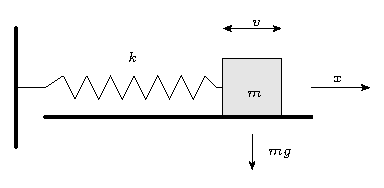
\includegraphics[width=0.5\textwidth]{task-oszillator_auf_rauer_unterlage-sketch.pdf}
  \end{figure}
  Die Anfangsbedingungen der Bewegung zur Zeit $t=0$ seien $x(0)=x_0$ und $v(0)=0$.
  \begin{atiSubtasks}
    \item{
      Lösen Sie für die ganze erste Periode der Bewegung die Differentialgleichung
      \[
        m \timeSecondDerivative{x} = -kx \mp \mu mg\ ,
      \]
      wobei das obere Vorzeichen für $v>0$ und das untere für $v<0$ gilt.
      Wie beeinflusst die Reibung die Schwingungsfrequenz?

      \begin{atiNote}
        Führen Sie die Differentialgleichung mithilfe der neuen Variablen
        \[
          \xi = x\pm \frac{\mu g}{\omega_0^2}
        \]
        auf die Gleichung des harmonischen Oszillators zurück.
      \end{atiNote}
    }
    \item{
      Geben Sie durch Verallgemeinerung Ihres Resultates $x(t)$ und $v(t)$ für die $n$-te Halbperiode für alle $n\in\setNatural$ an.
    }
    \item{
      Untersuchen Sie die Abnahme der Amplituden in aufeinanderfolgenden Perioden und zeigen Sie, dass die Maxima und Minima der Funktion $x(t)$ auf Geraden liegen.
      Bestimmen Sie die Gleichungen dieser Geraden.
      Skizzieren Sie den Verlauf der gedämpften Schwingung.
    }
  \end{atiSubtasks}
\end{atiTask}
	\import{database/mathematische_methoden_der_physik_i/ordinary_deq/inhomogenous_deq/}{task-oszillator_auf_rauer_unterlage}


	% \begin{atiTask}[
  title = Die Methode der unbestimmten Koeffizienten
]
  Lösen Sie die folgenden Differentialgleichungen mithilfe der Methode der unbestimmten Koeffizienten für die nebenstehenden Anfangsbedingungen.
  Führen Sie eine Probe durch.
  \begin{atiSubequations}
    \item{
      3y'' - 6y' - 24y = 72x^2 - 12x - 6
      \separate
      y(0) = -1
      \separate
      y'(0) = 8
    }
    \item{\locallabel{c}
      y'' + y' + y = (2+x)\cos x
      \separate
      y(0) = -1
      \separate
      y'(0) = 1
    }
    \item{\locallabel{d}
      y'' + y' + y = 2+x + \cos x
      \separate
      y(0) = -7
      \separate
      y'(0) = 8
    }
    \item{\locallabel{e}
      y^{(3)} - 12y' + 16y = 32x - 8
      \separate
      y(0) = -
      \separate
      y'(0) = 1
      \separate
      y''(0) = -28
    }
    \item{
      y'' - 9y = e^{3x}
      \separate
      y(0) = 3
      \separate
      y'(0) = \frac{55}{6}
    }
  \end{atiSubequations}
  \begin{atiNote}
    \begin{atiItems}
      \item[zu \localref{c}:]{
        Verwenden Sie einen Ansatz der Form
        \[
          y_\text{p} = \roundBrackets{a_0 + a_1 x}\sin x + \roundBrackets{b_0 + b_1 x}\cos x
        \]
      }
      \item[zu \localref{d}:]{
        Bestimmen Sie nur eine neue Partikulärlösung.
        Die homogene Lösung kann aus \localref{c} übernommen werden.
      }
      \item[zu \localref{e}:]{
        Überlegen Sie sich, wie der Ansatz für Differentialgleichungen zweiter Ordnung auf solche dritter Ordnung erweitert werden kann.
      }
    \end{atiItems}
  \end{atiNote}
\end{atiTask}
	% \bigskip
	% \begin{atiTask}[
  title = Gekoppelte Differentialgleichungen
]
  Betrachten Sie folgendes System von miteinander gekoppelten Differentialgleichungen erster Ordnung für die Funktionen $x(t)$ und $y(t)$.
  \[
    \tdrv{x} = \fdrv{x(t)}{t} = x + y + t\separate \tdrv{y} = \fdrv{y(t)}{t} = 3x - y
  \]
  Bestimmen Sie die Lösungen, indem Sie die beiden Gleichungen erster Ordnung in eine Gleichung zweiter Ordnung überführen.
  Finden Sie die spezielle Lösung mit den Anfangsbedingungen $x(0)=-\frac{1}{4}$ und $y(0)=1$ und führen Sie eine Probe durch.

  \begin{atiNote}
    Eliminieren Sie dazu $y$.
  \end{atiNote}
\end{atiTask}
	% \newpage
	% \begin{atiTask}[
  title = Die Variation der Konstanten
]
  Betrachten Sie die Differentialgleichung
  \[
    y'' + 5y' + 4y = \cos 2x \ .
  \]
  \begin{atiSubtasks}
    \item{
      Bestimmen Sie zunächst die Fundamentallösungen $y_1$ und $y_2$ der homogenen Gleichung.
    }
    \item{
      Variieren Sie die beiden Konstanten in
      \[
        y_\m{h} = c_1e^{-4x} + c_2e^{-x} \ ,
      \]
      indem Sie diese durch Funktionen $u(x)$ und $v(x)$ ausdrücken.
      Berechnen Sie die erste und die zweite Ableitung.
    }
    \item{
      Setzen Sie die dadurch erhaltenen Funktionen in die inhomogene Differentialgleichung ein und vereinfachen Sie die daraus resultierende Gleichung, indem Sie benutzen, dass $y_1$ und $y_2$ die homogene Differentialgleichung lösen.
    }
    \item{
      Vereinfachen Sie die Gleichung weiter, indem Sie fordern, dass
      \begin{equation}
        \locallabel{equ1}
        u'(x)e^{-4x} + v'(x)e^{-x} = 0
      \end{equation}
      gilt.
      Begründen Sie, warum diese Forderung zulässig ist.
    }
    \item{
      Leiten Sie aus der Gleichung \localref{equ1} eine weitere Bedingung ab, die Ihnen bei der Vereinfachung hilft.
    }
    \item{
      Sie erhalten nun eine einfachere Form der ursprünglichen Differentialgleichung
      \begin{equation}
        \locallabel{equ2}
        -4u'(x)e^{-4x} - v'(x)e^{-x} = \cos 2x
      \end{equation}
      Bestimmen Sie ausgehend von den Gleichungen \localref{equ1} und \localref{equ2} die Funktionen $u$ und $v$.
    }
    \item{
      Führen Sie eine Probe für die so erhaltene allgemeine Lösung durch.
    }
  \end{atiSubtasks}
\end{atiTask}

	% \begin{atiTask}[
	title = Die charakteristische Gleichung,
	topic = Gewöhnliche Differentialgleichungen,
	subtopic = Die lineare homogene Differentialgleichung 2. Ordnung mit konstanten Koeffizienten,
	language = Deutsch,
]
	Konstruieren Sie für jede der beiden folgenden Differentialgleichungen deren allgemeine Lösung und bestimmen Sie die spezielle Lösung, die den nebenstehenden Anfangsbedingungen genügt.
	\begin{atiSubequations}
		\item{
			y'' - 2y' + y = 0 \separate y(1) = 2 \separate y(0) = 1
		}
		\item{
			y'' + 6y' + 13y = 0 \separate y(0) = 3 \separate y'(0) = 7
		}
	\end{atiSubequations}
	Machen Sie in beiden Fällen für die allgemeine Lösung die Probe durch Einsetzen in die ursprüngliche Differentialgleichung.
\end{atiTask}
	% \bigskip
	% \begin{atiTask}[
  title = Die Wronski-Determinante
]
  \begin{atiSubtasks}
    \item{
      Drücken Sie die Ableitung $W'$ der Wronski-Determinante
      \[
        W(x) = y_1(x)y'_2(x)-y_2(x)y'_1(x)
      \]
      mithilfe der Differentialgleichung
      \[
        ay'' + by' + cy = 0
      \]
      durch die Wronski-Determinante selbst aus.
    }
    \item{
      Lösen Sie die so entstehende gewöhnliche Differentialgleichung für $W$.
      Zeigen Sie anhand dieser Lösung die folgende Aussage.
      \[
        \exists x\in\setReal\colon W(x) \neq 0 \iff \forall x\in\setReal\colon W(x) \neq 0
      \]
    }
    \item{
      Betrachten Sie nun eine lineae Differentialgleichung zweiter Ordnung mit nicht konstanten Koeffizienten.
      \[
        y'' + p(x)y' + q(x)y = 0
      \]
      Geben Sie die zugehörige Wronski-Determinante an.
    }
    \item{
      Bestimmen Sie mit diesem Verfahren die Wronski-Determinante der Differentialgleichung
      \[
        y'' + \frac{1}{x}y' - \frac{m^2}{x^2}y = 0
      \]
    }
    \item{
      \textbf{Zusatz:}
      Überzeugen Sie sich, dass $y_1(x)=x^m$ eine Lösung der Gleichung ist.
      Konstruieren Sie eine zweite Lösung aus dem Ansatz $y_2(x) = u(x)y_1(x)$, indem Sie eine Differentialgleichung für $u(x)$ aufstellen und diese durch zweimalige Integration lösen.
      Überprüfen Sie durch Einsetzen, dass auch $y_2$ eine Lösung der obigen Differentialgleichung ist.
    }
  \end{atiSubtasks}
\end{atiTask}
	% \bigskip
	% \begin{atiTask}[
	title = Die homogene Euler-Gleichung,
	topic = Gewöhnliche Differentialgleichungen,
	subtopic = Die lineare homogene Differentialgleichung 2. Ordnung mit konstanten Koeffizienten,
	language = Deutsch,
]
	Die Eulersche Differentialgleichung ist durch die folgende Form gegeben.
	Dabei stellen die Koeffizienten $a$,$b$ und $c$ reelle Konstanten dar.
	\[
		ax^2y'' + bxy' + cy = 0
	\]
	\begin{atiSubtasks}
		\item{
			Überführen Sie diese Differentialgleichung mithilfe der Substitution $x = e^{t(x)}$ in eine Differentialgleichung mit konstanten Koeffizienten.
		}
		\item{
			Ein wichtiges Beispiel für die Potentialtheorie stellt die folgende Differentialgleichung dar.
			Dabei beschreibt $n$ eine nichtnegative reelle Konstante, $r$ eine nichtnegative reelle Variable und $R$ eine Funktion, welche von $r$ abhängt.
			\[
				\nfdrv[2]{R}{r} + \frac{2}{r}\nfdrv{R}{r} - \frac{n(n+1)}{r^2}R = 0
			\]
			\begin{atiSubsubtasks}
				\item{
					Behandeln Sie die genannte Differentialgleichung nach der zuvor beschriebenen Methode.
				}
				\item{
					Konstruieren Sie die allgemeine Lösung $R$ der entstehenden Differentialgleichung mit konstanten Koeffizienten.
				}
				\item{
					Geben Sie diejenige spezielle Lösung an, welche die folgende Bedingung erfüllt.
					\[
						R\conv[r\conv\infty]0
					\]
				}
			\end{atiSubsubtasks}
		}
		\item{
			\textbf{Zusatz:}
			Lösen Sie mit derselben Methode die folgende Differentialgleichung.
			\[
				x^2y'' - xy' + 10y = 0
			\]
		}
	\end{atiSubtasks}
\end{atiTask}

	% \newpage
	% \begin{atiTask}[
	title = Die Wronski-Determinante
]
	Gegeben sei die folgende Differentialgleichung, wobei $p$ und $q$ Funktionen in Abhängigkeit von $x$ darstellen.
	Weiterhin seien $y_1$ und $y_2$ zwei Lösungen dieser Gleichung.
	\[
		y'' + p(x)y' + q(x)y = 0
	\]
	\begin{atiSubtasks}
		\item{\locallabel{a}
			Zeigen Sie, dass die Wronski-Determinante $W$ der folgenden separablen Differentialgleichung genügt und lösen Sie diese Gleichung durch Trennung der Variablen.
			\[
				W' = -p(x)\cdot W
			\]
			Damit ist es möglich die Wronski-Determinante direkt aus der zugehörigen Differentialgleichung ohne Kenntnis der Lösung dieser zu bestimmen.
		}
		\item{
			Es sei die Lösung $y_1$ bereits bekannt.
			Interpretieren Sie die folgende Gleichung als inhomogene Differentialgleichung erster Ordnung für $y_2$ und lösen Sie diese durch Variation der Konstanten.
			\[
				y_1(x)y_2'(x)-y_2(x)y_1'(x) = W(x)
			\]
			So können Sie die zweite Fundamentallösung aus der Kenntnis der ersten Fundamentallösung und der Wronski-Determinante bestimmen.
		}
		\item{
			Betrachten Sie die folgende Differentialgleichung mit den reellen konstanten Koeffizienten $a$, $b$ und $c$.
			\[
				ay'' + by' + cy = 0
			\]
			\begin{atiSubsubtasks}
				\item{
					Bestimmen Sie die Wronski-Determinante dieser Differentialgleichung mit der in \localref{a} beschriebenen Methode.
				}
				\item{
					Nehmen Sie an, dass die folgende Lösung bekannt ist, und bestimmen Sie durch Verwendung des zuvor beschriebenen Verfahrens die zweite Fundamentallösung.
					\[
						y_1(x) = e^{\lambda_1 x}
						\separate
						\lambda_1 \define -\frac{b}{2a} + \frac{1}{2a}\sqrt{b^2-4ac}
					\]
				}
			\end{atiSubsubtasks}
		}
		\item{
			\textbf{Für Interessierte:}
			Gegeben sei die folgende Differentialgleichung mit der reellen Konstanten $m$.
			\[
				y'' + \frac{1}{x} y' - \frac{m^2}{x}y = 0
			\]
			\begin{atiSubsubtasks}
				\item{
					Bestimmen Sie die Wronski-Determinante dieser Differentialgleichung.
				}
				\item{
					Überzeugen Sie sich, dass die folgende Funktion eine Lösung dieser Differentialgleichung ist und berechnen Sie nach dem zuvor beschriebenen Verfahren die zweite Fundamentallösung.
					\[
						y_1(x) = x^m
					\]
					Machen Sie die Probe für diese zweite Lösung und geben Sie auch die allgemeine Lösung der Differentialgleichung an.
				}
			\end{atiSubsubtasks}
		}
	\end{atiSubtasks}
\end{atiTask}

	% \begin{atiTask}[
  title = Der integrierende Faktor
]
  Untersuchen Sie die folgenden Differentialgleichungen auf Exaktheit.
  % und lösen Sie die nicht-exakten Differentialgleichungen.
  \begin{atiSubequations}
    \item{
      \curvb{x+y}x^2y' + xy^2 + 3x^2y = 0
    }
    \item{
      yx^3 - 2x^4 = \curvb{3y^2x^3-x^4} y'
    }
    \item{
      \curvb{x\cos y - xy\sin y}y' + 2y\cos y + x = 0
    }
  \end{atiSubequations}
  Berechnen Sie die allgemeinen Lösungen der nicht-exakten Differentialgleichungen in impliziter Form, indem Sie die folgende Anleitung verwenden.
  \begin{atiItems}
    \item{
      Bestimmen Sie einen integrierenden Faktor, der nur von der ersten freien Variable abhängt.
    }
    \item{
      Notieren Sie die neue, mit dem integrierenden Faktor multiplizierte, Differentialgleichung.
    }
    \item{
      Zeigen Sie die Exaktheit der neuen Differentialgleichung.
    }
    \item{
      Lösen Sie die neue Differentialgleichung durch das Auffinden einer Potentialfunktion.
    }
    \item{
      Führe Sie die Probe durch, indem Sie die erhaltene Lösung implizit differenzieren und auf die ursprüngliche Differentialgleichung zurückführen.
    }
  \end{atiItems}
  % \begin{atiSubtasks}
  %   \item{
  %     Überprüfen Sie, ob die gegebenen Differentialgleichungen exakt sind.
  %   }
  %   \item{
  %     Lösen Sie die nicht-exakten Differentialgleichungen, indem Sie nach der folgenden Anleitung vorgehen.
  %     \begin{atiItems}
  %       \item{
  %         Bestimmen Sie einen integrierenden Faktor, der nur von der ersten freien Variable $x$ abhängt.
  %       }
  %       \item{
  %         Überprüfen Sie die Exaktheit der mit dem integrierenden Faktor multiplizierten Differentialgleichung.
  %       }
  %       \item{
  %         Lösen Sie nun die mit dem integrierenden Faktor multiplizierte Differentialgleichung durch das Auffinden einer Potentialfunktion.
  %       }
  %       \item{
  %         Führe Sie die Probe durch, indem Sie Ihre Lösung implizit differenzieren und auf die ursprüngliche Differentialgleichung zurückführen.
  %       }
  %     \end{atiItems}
  %   }
  % \end{atiSubtasks}
\end{atiTask}
	% \begin{atiTask}[
  title = Spezielle integrierende Faktoren
  ]
  Es sei die folgende Differentialgleichung für stetig differenzierbare Funktionen $\func{A,B}{\setR^2}{\setR}$ gegeben.
  \[
    A(x,y) + B(x,y)y' = 0
  \]
  \begin{atiSubtasks}
    \item{
      Zeigen Sie durch die Verwendung der Integrabilitätsbedingung, dass wenn es eine Funktion $\func{f}{\setR}{\setR}$ gibt, sodass das Folgende gilt, so
      \[
        f(xy) = \frac{\partial_1B(x,y) - \partial_2A(x,y)}{xA(x,y)-yB(x,y)}
      \]
    }
  \end{atiSubtasks}
\end{atiTask}
	% \bigskip
	% \begin{atiTask}[
  title = Konstruktion eines integrierenden Faktors
]
  Wir wenden uns noch einmal der folgenden Differentialgleichung zu.
  \[
     y' - y + 3x^2y^3 = 0
  \]
  Konstruieren Sie nun einen integrierenden Faktor $\Lambda(x,y)$ auf zwei Wegen.
  \begin{atiSubtasks}
    \item{
      Sie haben diese Differentialgleichung in der zweiten Aufgabe der dritten Übungsserie mit der Substitution $z = y^{-2}$ in eine lineare Differentialgleichung überführt, die auch nicht exakt ist.
      Bestimmen Sie zuerst für diese Gleichung einen integrierenden Faktor $\lambda(x)$, der nur von der Variablen $x$ abhängt.
      Dieser Faktor allein macht die ursprüngliche Differentialgleichung noch nicht exakt.
      Ermitteln Sie nun für die mit $\lambda(x)$ multiplizierte ursprüngliche Gleichung einen integrierenden Faktor $\mu(y)$, der nur von der Variablen $y$ abhängt.
    }
    \item{
      Machen Sie von vornherein für den integrierenden Faktor $\Lambda(x,y)$ der ursprünglichen Differentialgleichung den Produktansatz $\Lambda(x,y)=\lambda(x)\cdot\mu(y)$ und bestimmen Sie die Funktionen $\lambda(x)$ und $\mu(y)$ ohne Rückgriff auf die in der Variablen $z$ lineare Differentialgleichung.
    }
    \item{
      \textbf{Zusatz:}
      Weisen Sie nach, dass die Ausgangsgleichung mit diesem integrierenden Faktor $\Lambda(x,y)$ exakt ist und lösen Sie diese.
      Vergleichen Sie das Ergebnis mit dem vorherigen Resultat aus der zweiten Aufgabe der dritten Übungsserie.
    }
  \end{atiSubtasks}
\end{atiTask}
	% \bigskip
	% \begin{atiTask}[
  title = Ideales Gas
]
  Ein ideales Gas befinde sich in einem Kolben, der zusammengepresst wird.
  Dabei gelten die folgenden Zustandsgleichungen.
  \[
    pV = Nk_\text{B}T
    \separate
    E = \frac{3}{2}Nk_\text{B}T
  \]
  Darin steht $p$ für den Druck, $V$ für das Volumen, $N$ für die Teilchenanzahl, $T$ für die Temperatur, $E$ für die innere Energie und $k_\text{B}$ für die Boltzmann-Konstante.
  Nach dem ersten Hauptsatz der Thermodynamik ändert sich die innere Energie $E$ durch das Verrichten von Arbeit $p\,\infinitesimal V$ und die Abgabe von Wärme $\delta Q$.
  \[
    \infinitesimal E = \delta Q - p\,\infinitesimal V
  \]
  \begin{atiSubtasks}
    \item{
      Schon die Schreibweise $\delta Q$ (anstelle von $\infinitesimal Q$) deutet an, dass es keine Funktion $Q(V,T)$ mit dem totalen Differential $\delta Q$ gibt.
      Bestätigen Sie diese Aussage, indem Sie die Integrabilitätsbedingung überprüfen.
    }
    \item{
      Suchen Sie nun einen integrierenden Faktor $\lambda$, der nur von $T$ abhängt, sodass $\infinitesimal S = \lambda\,\delta Q$ ein totales Differential beschreibt.
    }
    \item{
      Führen Sie eine Probe durch, indem Sie nun für $\infinitesimal S$ die Integrabilitätsbedingung nachprüfen.
    }
  \end{atiSubtasks}
\end{atiTask}
	% \begin{atiTask}[
	title = Integrierende Faktoren,
	topic = Gewöhnliche Differentialgleichungen,
	subtopic = Exakte Differentialgleichungen: Der integrierende Faktor,
	language = Deutsch
]
	\begin{atiSubtasks}
		\item{
			Die folgende Differentialgleichung sei gegeben.
			\[
				A(x,y) + B(x,y)y' = 0
			\]
			Zeigen Sie durch Verwendung der Integrabilitätsbedingung die beiden folgenden Aussagen.
			\begin{atiItems}
				\item{
					Kann der folgende Ausdruck als eine Funktion $f$ der Variablen $z(x,y)\define xy$ geschrieben werden, so hängt auch der integrierende Faktor $\lambda$ nur von dieser Variable $z$ ab.
					\[
						\frac{1}{xA(x,y)-yB(x,y)}\curvb{\partial_x B(x,y) - \partial_y A(x,y)}
					\]
					Geben Sie den Zusammenhang von $\lambda$ und $f$ an.
				}
				\item{
					Kann der folgende Ausdruck als eine Funktion $g$ der Variablen $w(x,y)\define x + y$ geschrieben werden, so hängt auch der integrierende Faktor $\lambda$ nur von dieser Variable $z$ ab.
					\[
						\frac{1}{A(x,y)-B(x,y)}\curvb{\partial_x B(x,y) - \partial_y A(x,y)}
					\]
					Geben Sie den Zusammenhang von $\lambda$ und $g$ an.

				}
			\end{atiItems}
		}
		\item{
			Eine der beiden zuvor genannten Eigenschaften trifft auf eine der beiden folgenden Differentialgleichungen zu.
			Finden Sie diesen Fall heraus und berechnen Sie einen integrierenden Faktor mit dem Ergebnis aus dem vorherigen Aufgabenteil.
			\begin{atiSubequations}
				\item{
					(xy-1) + \curvb{x^2-xy}y' = 0
				}
				\item{
					y + \curvb{x - 2x^2y^3}y' = 0
				}
			\end{atiSubequations}
			Lösen Sie die Differentialgleichung mit diesem integrierenden Faktor und machen Sie anschließend die Probe anhand der ursprünglichen Differentialgleichung.
			Die Lösung der verbleibenden Differentialgleichung ist nicht verlangt.
		}
	\end{atiSubtasks}
\end{atiTask}

	% \begin{atiTask}[
  title = Freier Fall mit Reibung
]
 Beim freien Fall mit Fallbeschleunigung $g\in\setR^+$ unter dem Einfluss einer geschwindigkeitsproportionalen Reibungskraft mit Reibungskoeffizient $\gamma\in\setR^+$ genügt die abwärts gerichtete Geschwindigkeitsfunktion $v$ eines Massenpunktes mit Masse $m\in\setR^+$ der folgenden Differentialgleichung.
 \[
   m\tdrv{v} + \gamma v = mg
 \]
 \begin{atiSubtasks}
   \item{\locallabel{a}
    Lösen Sie diese Differentialgleichung durch die Methode der Variation der Konstanten und bestimmen Sie eine Lösung, die den Anfangsbedingungen $t_0\define 0$ und $v_0\define v(t_0)=0$ genügt.
  }
  \item{\locallabel{b}
    Berechnen Sie die stationäre Endgeschwindigkeit $v_\infty$ mithilfe der folgenden Definition und der Lösung der Differentialgleichung.
    \[
      v_\infty \define \lim_{t\conv\infty}v(t)
    \]
    Berechnen Sie ein zweites Mal $v_\infty$ unter der Annahme, dass die Lösung des Anfangswertproblems nicht bekannt ist.
    Betrachten Sie hierfür den Grenzwert der Differentialgleichung.
  }
  \item{\locallabel{c}
    \textbf{Zusatz:}
    Lösen Sie noch einmal die Differentialgleichung des freien Falls durch die Methode der Trennung der Variablen.
  }
 \end{atiSubtasks}
\end{atiTask}
\begin{atiSolution}
  \begin{atiSubtaskSolutions}
    \item[\localref{a}]{
      Die zur gegebenen Differentialgleichung zugehörigen homogene Differentialgleichung kann durch die folgende Form beschrieben werden.
      \[
        m\tdrv{v} + \gamma v = 0 \implies \tdrv{v} = -\frac{\gamma}{m}v\atiPoints[\frac{1}{2}]
      \]
      Diese Formel lässt sich separieren und durch die Methode der Trennung der Variablen lösen.
      \[
        \frac{\tdrv{v}(t)}{v(t)} = -\frac{\gamma}{m} \implies \integral{t_0}{t}{\frac{\tdrv{v}(t)}{v(t)}}{t} = \integral{v_0}{v(t)}{\frac{1}{s}}{s} = -\integral{t_0}{t}{\frac{\gamma}{m}}{t}\atiPoints[\frac{1}{2}]
      \]
      \[
        \implies \ln\curvb{\frac{v(t)}{v_0}} = -\frac{\gamma}{m}(t-t_0) \implies v(t) = v_0 e^{-\frac{\gamma}{m}(t-t_0)}\atiPoints[\frac{1}{2}]
      \]
      Nach der Methode der Variation der Konstanten gehen wir nun davon aus, dass sich die Lösung der ursprünglichen Differentialgleichung durch die folgende Funktion beschreiben lässt.
      \[
        v(t) = \varphi(t)e^{-\frac{\gamma}{m}(t-t_0)}\atiPoints[\frac{1}{2}]
      \]
      \[
        \implies \tdrv{v}(t) = \tdrv{\varphi}(t)e^{-\frac{\gamma}{m}(t-t_0)} - \varphi(t)\frac{\gamma}{m}e^{-\frac{\gamma}{m}(t-t_0)}\atiPoints[\frac{1}{2}]
      \]
      Das Einsetzen der Ableitung in die ursprüngliche Differentialgleichung ergibt dann das Folgende.
      \[
        m\tdrv{\varphi}(t)e^{-\frac{\gamma}{m}(t-t_0)} = mg \implies \tdrv{\varphi}(t) = ge^{\frac{\gamma}{m}(t-t_0)}\atiPoints[\frac{1}{2}]
      \]
      \[
        \implies \varphi(t) = \frac{mg}{\gamma}e^{\frac{\gamma}{m}(t-t_0)} - \frac{mg}{\gamma} + \varphi(t_0)
      \]
      \[
        \implies v(t) = \varphi(t)e^{-\frac{\gamma}{m}(t-t_0)} = \frac{mg}{\gamma}\boxb{1 - e^{-\frac{\gamma}{m}(t-t_0)}} + \varphi(t_0)e^{-\frac{\gamma}{m}(t-t_0)} \atiPoints[\frac{1}{2}]
      \]
      Zu beachten ist hier, dass $v_0 = v(t_0) = \varphi(t_0)$ gilt.
      Die Lösung des Anfangswertproblems ist damit wegen $t_0=0$ und $v_0=0$ gegeben durch die folgende Funktion.
      \[
        v(t) = \frac{mg}{\gamma}\curvb{1-e^{-\frac{\gamma}{m}t}}\atiPoints[\frac{1}{2}]
      \]
    }
    \item[\localref{b}]{
      Die stationäre Endgeschwindigkeit lässt sich nun einfach mithilfe des Limes berechnen.
      \[
        v_\infty = \lim_{t\conv\infty}v(t) = \lim_{t\conv\infty} \frac{mg}{\gamma}\curvb{1-e^{-\frac{\gamma}{m}t}} = \frac{mg}{\gamma}\curvb{1-\lim_{t\conv\infty}e^{-\frac{\gamma}{m}t}} = \frac{mg}{\gamma} \atiPoints[1]
      \]
      Ohne die Kenntnis der Lösung lässt sich nun das Folgende notieren.
      \[
        \lim_{t\conv\infty}\boxb{m\tdrv{v}(t) + \gamma v(t)} = \lim_{t\conv\infty}mg \implies m\lim_{t\conv\infty}\tdrv{v}(t) + \gamma \lim_{t\conv\infty}v(t) = mg
      \]
      Da der Limes existiert und $v$ eine stetig differenzierbare Funktion ist, muss demnach das Folgende gelten.
      \[
        \lim_{t\conv\infty}\tdrv{v}(t)=0 \implies v_\infty = \lim_{t\conv\infty}v(t) = \frac{mg}{\gamma} \atiPoints[1]
      \]
    }
    \item[\localref{c}]{
      Die in der Aufgabe gegebene Differentialgleichung ist separierbar und damit durch die Methode der Trennung der Variablen lösbar.
      \[
        \tdrv{v}(t) = g-\frac{\gamma}{m}v(t) \implies \frac{\tdrv{v}(t)}{g-\frac{\gamma}{m}v(t)} = 1 \implies \integral{t_0}{t}{\frac{\tdrv{v}(t)}{g-\frac{\gamma}{m}v(t)}}{t} = \integral{t_0}{t}{}{t} \atiPoints[+\frac{1}{2}]
      \]
      \[
        \implies -\frac{m}{\gamma}\ln\boxb{\frac{g-\frac{\gamma}{m}v(t)}{g-\frac{\gamma}{m}v_0}} = t-t_0
      \]
      \[
        \implies v(t) = \frac{m}{\gamma}\boxb{g - \curvb{g-\frac{\gamma}{m}v_0}e^{-\frac{\gamma}{m}(t-t_0)}}
      \]
      \[
        \implies v(t) = \frac{mg}{\gamma}\boxb{1-e^{-\frac{\gamma}{m}(t-t_0)}} + v_0e^{-\frac{\gamma}{m}(t-t_0)}\atiPoints[+\frac{1}{2}]
      \]
    }
  \end{atiSubtaskSolutions}
\end{atiSolution}
	% \bigskip
	% \begin{atiTask}[
  title = Exakte Differentialgleichungen
]
  \begin{atiSubtasks}
    \item{\locallabel{a}
      Zeigen Sie, dass die folgenden Differentialgleichungen exakt sind, und lösen Sie diese durch das Auffinden einer Potentialfunktion.
      \begin{atiSubequations}
        \item{\locallabel{ai}
          \curvb{x+y^3}y' + y = x^3
        }
        \item{\locallabel{aii}
          0 = \sin\curvb{xy^2} + xy^2\cos\curvb{xy^2} + \boxb{2x^2y\cos\curvb{xy^2} + 2y}y'
        }
      \end{atiSubequations}
    }
    \item{\locallabel{b}
      Zeigen Sie, dass es sich bei den folgenden Gleichungen um nicht exakte Differentialgleichungen handelt, indem Sie die Integrabilitätsbedingung überprüfen.
      \begin{atiSubequations}
        \item{\locallabel{bi}
          0 = 2\cos y + 4x^2y\sin y + \curvb{yx^3\cos y + x^3\sin y}y' - xy'\sin y
        }
        \item{\locallabel{bii}
          x\arctan\curvb{\frac{x}{y^2}} + \frac{x^2y^2}{x^2+y^4} = \frac{2x^3y}{x^2+y^4}y'
        }
      \end{atiSubequations}
    }
  \end{atiSubtasks}
\end{atiTask}
\begin{atiSolution}
  \begin{atiSubtaskSolutions}
    \item[\localref{a}]{
      \begin{atiSubtaskSolutions}
        \item[\localref{ai}]{
          Wir definieren zwei Funktionen $\func{f,g}{\setR^2}{\setR}$, sodass für alle $x,y\in\setR$ folgende Gleichungen gelten.
          \[
            f(x,y)\define y-x^3\separate g(x,y)\define x+y^3
          \]
          \[
            \implies f(x,y) + g(x,y)y' = 0
          \]
          Die Integrabilitätsbedingung ist nach der folgenden Aussage für alle $x,y\in\setR$ erfüllt.
          Die Differentialgleichung ist damit exakt.
          \[
            \partial_2f(x,y) = \pdrvopb{\tilde{y}}{f(x,\tilde{y})}{y} = 1 = \pdrvopb{\tilde{x}}{g(\tilde{x},y)}{x} = \partial_1g(x,y)
          \]
          Es gibt nun eine zweimal stetig differenzierbare Potentialfunktion $\func{\varphi}{\setR^2}{\setR}$, die die folgende Bedingung erfüllt.
          \[
            \partial_1\varphi = f \separate \partial_2\varphi = g
          \]
          Um diese zu berechnen, kann man zum Beispiel einen der beiden folgenden Wege verwenden.
          \[
            \varphi(x,y) = \iintegralb{\partial_1\varphi(s,y)}{s}{x} = \iintegralb{f(s,y)}{s}{x} = yx - \frac{x^4}{4} + c(y)
          \]
          \[
            \implies \partial_2\varphi(x,y) = x + c'(y) = g(x,y) = x + y^3
          \]
          \[
            \implies c'(y) = y^3 \implies c(y) = \frac{y^4}{4} + K
          \]
          \[
            \implies \varphi(x,y) = xy - \frac{x^4}{4} + \frac{y^4}{4} + K
          \]
          \[
            \varphi(x,y) = \iintegralb{\partial_2\varphi(x,s)}{s}{y} = \iintegralb{g(x,s)}{s}{y} = xy + \frac{y^4}{4} + d(x)
          \]
          \[
            \implies \partial_1\varphi(x,y) = y + d'(x) = f(x,y) = y - x^3
          \]
          \[
            \implies d'(x) = -x^3 \implies d(x) = -\frac{x^4}{4} + K
          \]
          \[
            \implies \varphi(x,y) = xy - \frac{x^4}{4} + \frac{y^4}{4} + K
          \]
          Jetzt gehen wir davon aus, dass es sich bei $y$ um eine stetig differenzierbare Funktion handelt.
          Nach Verwendung der Kettenregel und der gegebenen Differentialgleichung können wir auf das Folgende für alle $x$ einer offenen Teilmenge $U\subset\setR$ schließen.
          \[
            \fdrvopb{s}{\varphi(s,y(s))}{x} = \partial_1\varphi(x,y(x)) + \partial_2\varphi(x,y(x)) y'(x) = 0
          \]
          Dies ist nur dann möglich, wenn es für alle $x\in U$ eine Konstante $C\in\setR$ gibt, sodass das Folgende gilt.
          \[
            \varphi(x,y(x)) = C = xy(x) - \frac{x^4}{4} + \frac{y^4(x)}{4} + K
          \]
          Dies ist auch gleichzeitig die Funktion $y$ in impliziter Form.
        }
        \item[\localref{aii}]{
          Wir definieren zwei Funktionen $\func{f,g}{\setR^2}{\setR}$, sodass für alle $x,y\in\setR$ folgende Gleichungen gelten.
          \[
            f(x,y) \define \sin\curvb{xy^2} + xy^2\cos\curvb{xy^2} \separate g(x,y) \define 2x^2y\cos\curvb{xy^2} + 2y
          \]
          \[
            \implies f(x,y) + g(x,y)y' = 0
          \]
          Die Integrabilitätsbedingung ist nach der folgenden Aussage für alle $x,y\in\setR$ erfüllt.
          Die Differentialgleichung ist damit exakt.
          \[
            \partial_2f(x,y) = \pdrvopb{\tilde{y}}{f(x,\tilde{y})}{y} = 4xy\cos\curvb{xy2} - 2x^2y^3\sin\curvb{xy^2} = \pdrvopb{\tilde{x}}{g(\tilde{x},y)}{x} = \partial_1g(x,y)
          \]
          Es gibt nun eine zweimal stetig differenzierbare Potentialfunktion $\func{\varphi}{\setR^2}{\setR}$, die die folgende Bedingung erfüllt.
          \[
            \partial_1\varphi = f \separate \partial_2\varphi = g
          \]
          Um diese zu berechnen, kann man zum Beispiel einen der beiden folgenden Wege verwenden.
          \[
            \varphi(x,y) = \iintegralb{\partial_1\varphi(s,y)}{s}{x} = \iintegralb{f(s,y)}{s}{x} = -\frac{\cos\curvb{xy^2}}{y^2} + c(y)
          \]
          \[
            \implies \partial_2\varphi(x,y) = + c'(y) = g(x,y) =
          \]
          \[
            \implies c'(y) = y^3 \implies c(y) = \frac{y^4}{4} + K
          \]
          \[
            \implies \varphi(x,y) = xy - \frac{x^4}{4} + \frac{y^4}{4} + K
          \]
          \[
            \varphi(x,y) = \iintegralb{\partial_2\varphi(x,s)}{s}{y} = \iintegralb{g(x,s)}{s}{y} = xy + \frac{y^4}{4} + d(x)
          \]
          \[
            \implies \partial_1\varphi(x,y) = y + d'(x) = f(x,y) = y - x^3
          \]
          \[
            \implies d'(x) = -x^3 \implies d(x) = -\frac{x^4}{4} + K
          \]
          \[
            \implies \varphi(x,y) = xy - \frac{x^4}{4} + \frac{y^4}{4} + K
          \]
        }
      \end{atiSubtaskSolutions}
    }
    \item[\localref{b}]{
      \begin{atiSubtaskSolutions}
        \item[\localref{bi}]{
          Wir definieren zwei Funktionen $\func{f,g}{\setR^2}{\setR}$, sodass für alle $x,y\in\setR$ folgende Gleichungen gelten.
          \[
            f(x,y) \define 2\cos y + 4x^2y\sin y \separate g(x,y) \define yx^3\cos y + x^3\sin y - x\sin y
          \]
          \[
            \implies f(x,y) + g(x,y)y' = 0
          \]
          Wir überprüfen wieder die Integrabilitätsbedingung.
          Es gibt also $x,y\in\setR$, sodass die folgende Implikation gilt.
          \[
            \partial_2f(x,y) = \pdrvopb{\tilde{y}}{f(x,\tilde{y})}{y} = -2\sin y + 4x^2\sin y + 4x^2y\cos y
          \]
          \[
            \partial_1g(x,y) = \pdrvopb{\tilde{x}}{g(\tilde{x},y)}{x} = 3x^2y\cos y + 3x^2\sin y - \sin y
          \]
          \[
            \implies \partial_2f(x,y) - \partial_1g(x,y) = \curvb{x^2-1}\sin y + \curvb{1-3x^2}y\cos y \neq 0
          \]
          Die Integrabilitätsbedingung ist damit nicht erfüllt.
          Demzufolge ist diese Differentialgleichung nicht exakt.
        }
        \item[\localref{bii}]{
          Wir definieren zwei Funktionen $\func{f,g}{\setR\times\setR\setminus\set{0}}{\setR}$, sodass für alle $x,y\in\setR$ mit $y\neq 0$ folgende Gleichungen gelten.
          \[
            f(x,y) \define x\arctan\curvb{\frac{x}{y^2}} + \frac{x^2y^2}{x^2+y^4} \separate g(x,y) \define -\frac{2x^3y}{x^2+y^4}
          \]
          \[
            \implies f(x,y) + g(x,y)y' = 0
          \]
          Wir überprüfen wieder die Integrabilitätsbedingung.
          Es gibt also $x,y\in\setR$ mit $y\neq 0$, sodass die folgende Implikation gilt.
          \[
            \partial_2f(x,y) = \pdrvopb{\tilde{y}}{f(x,\tilde{y})}{y} = -\frac{4x^4y^5}{\curvb{x^2+y^4}^2}
          \]
          \[
            \partial_1g(x,y) = \pdrvopb{\tilde{x}}{g(\tilde{x},y)}{x} = -\frac{6x^2y}{x^2+y^4} + \frac{4x^4y}{\curvb{x^2+y^4}^2}
          \]
          % \[
          %   \pdrvopb{\tilde{x}}{g(\tilde{x},y)}{x} = -\frac{6x^2y}{x^2+y^4} + \frac{4x^4y}{\curvb{x^2+y^4}^2}
          % \]
          \[
            \implies \partial_2f(x,y) - \partial_1g(x,y) = \frac{6x^2y}{x^2+y^4} - \frac{8x^4y}{\curvb{x^2+y^4}^2} \neq 0
          \]
          Die Integrabilitätsbedingung ist damit nicht erfüllt.
          Demzufolge ist diese Differentialgleichung nicht exakt.
        }
      \end{atiSubtaskSolutions}
    }
  \end{atiSubtaskSolutions}
\end{atiSolution}
	% \newpage
	% \begin{atiTask}[
  title = Vollständiges Differential
]
  Es sei die folgende skalare Funktion für alle $x,y,z\in\setReal$ gegeben.
  \[
    \function{U}{\setReal^3}{\setReal}
    \separate
    U(x,y,z)\define x^4yz^2 + 2y^2x^3e^z
  \]
  \begin{atiSubtasks}
    \item{\locallabel{a}
      Bestimmen Sie das totale Differential $\infinitesimal U$ der Funktion $U$.
    }
    \item{\locallabel{b}
      Untersuchen Sie, ob es eine Funktion $\function{V}{\setReal^3}{\setReal}$ gibt, sodass das totale Differential $\infinitesimal V$ von $V$ für alle $x,y,z\in\setReal$ mit $x\neq 0$ die folgende Gleichung erfüllt.
      \[
        \infinitesimal V(x,y,z)\define \frac{1}{x^2} \infinitesimal U(x,y,z)
      \]
      \begin{atiNote}
        Überprüfen Sie dafür die Integrabilitätsbedingung des gegebenen Differentials.
      \end{atiNote}
    }
  \end{atiSubtasks}
\end{atiTask}
\begin{atiSolution}
  \begin{atiSubtaskSolutions}
    \item[\localref{a}]{
      Der Gradient der skalaren Funktion $U$ berechnet sich wie folgt, da es sich bei $U$ um eine stetig differenzierbare Funktion handelt.
      \[
        \nabla U(x,y,z) =
        \begin{pmatrix}
          \partial_1U(x,y,z) \\
          \partial_2U(x,y,z) \\
          \partial_3U(x,y,z)
        \end{pmatrix}
        =
        \begin{pmatrix}
          4x^3yz^2 + 6x^2y^2e^z \\
          x^4z^2 + 4x^3ye^z \\
          2x^4yz + 2x^3y^2e^z
        \end{pmatrix}
      \]
      Das totale Differential existiert, da sich $U$ zweimal stetig differenzieren lässt und damit durch den Satz von Schwarz die Integrabilitätsbedingung automatisch erfüllt ist.
      Es ist dann durch den folgenden Ausdruck gegeben.
      \[
        \infinitesimal U = \dotProduct{\nabla U}{\infinitesimal r}
        \separate
        \infinitesimal r \define
        \begin{pmatrix}
          \infinitesimal x \\
          \infinitesimal y \\
          \infinitesimal z
        \end{pmatrix}
      \]
      \[
        \implies \infinitesimal U(x,y,z) = \partial_1U(x,y,z)\infinitesimal x + \partial_2U(x,y,z)\infinitesimal y + \partial_3U(x,y,z)\infinitesimal z\atiPoints[1]
      \]
      \[
        \implies \infinitesimal U(x,y,z) = \roundBrackets{4x^3yz^2 + 6x^2y^2e^z}\infinitesimal x + \roundBrackets{x^4z^2 + 4x^3ye^z}\infinitesimal y + \roundBrackets{2x^4yz + 2x^3y^2e^z}\infinitesimal z \atiPoints[1]
      \]
    }
    \item[\localref{b}]{
      Für alle $x,y,z\in\setReal$ mit $x\neq 0$ gilt nun die folgende Aussage.
      Wir definieren hierfür die Funktionen $\function{f,g,h}{\setReal\setminus\set{0}{}\times\setReal^2}{\setReal}$.
      \[
        \frac{1}{x^2}\infinitesimal U(x,y,z) = \underbrace{\roundBrackets{4xyz^2 + 6y^2e^z}}_{\reverseDefine f(x,y,z)}\infinitesimal x + \underbrace{\roundBrackets{x^2z^2 + 4xye^z}}_{\reverseDefine g(x,y,z)}\infinitesimal y + \underbrace{\roundBrackets{2x^2yz + 2xy^2e^z}}_{\reverseDefine h(x,y,z)}\infinitesimal z
      \]
      Ein notwendiges (aber nicht hinreichendes) Kriterium für die Existenz der in der Aufgabenstellung beschriebenen Funktion $V$, ist die Erfüllung der Integrabilitätsbedingung.
      Es gibt nun $x,y,z\in\setReal$ mit $x\neq 0$, die die folgenden Implikationen erfüllen.
      \[
        \partial_2f(x,y,z) = \leibnizPartialDerivativeOperatorValue{s}{\roundBrackets{\frac{\partial_1U(x,s,z)}{x^2}}}{y} = \frac{\partial_2\partial_1U(x,y,z)}{x^2}
      \]
      \[
        \partial_1g(x,y,z) = \leibnizPartialDerivativeOperatorValue{s}{\roundBrackets{\frac{\partial_2U(s,y,z)}{s^2}}}{x} = \frac{\partial_2\partial_1U(x,y,z)}{x^2} - \frac{2\ \partial_2U(x,y,z)}{x^3}
      \]
      \[
        \implies \partial_2f(x,y,z) - \partial_1g(x,y,z) = \frac{2\ \partial_2U(x,y,z)}{x^3} = xz^2 + 4ye^z \neq 0
      \]
      \[
        \partial_3f(x,y,z) = \leibnizPartialDerivativeOperatorValue{s}{\roundBrackets{\frac{\partial_1U(x,y,s)}{x^2}}}{z} = \frac{\partial_3\partial_1U(x,y,z)}{x^2}
      \]
      \[
        \partial_1h(x,y,z) = \leibnizPartialDerivativeOperatorValue{s}{\roundBrackets{\frac{\partial_3U(s,y,z)}{s^2}}}{x} = \frac{\partial_3\partial_1U(x,y,z)}{x^2} - \frac{2\ \partial_3U(x,y,z)}{x^3}
      \]
      \[
        \implies \partial_3f(x,y,z) - \partial_1h(x,y,z) = \frac{2\ \partial_3U(x,y,z)}{x^3} = 2xyz + 2y^2e^z \neq 0
      \]
      \[
        \partial_3g(x,y,z) = \leibnizPartialDerivativeOperatorValue{s}{\roundBrackets{\frac{\partial_2U(x,y,s)}{x^2}}}{z} = \frac{\partial_3\partial_2U(x,y,z)}{x^2}
      \]
      \[
        \partial_2h(x,y,z) = \leibnizPartialDerivativeOperatorValue{s}{\roundBrackets{\frac{\partial_3U(x,s,z)}{x^2}}}{y} = \frac{\partial_2\partial_3U(x,y,z)}{x^2}
      \]
      \[
        \implies \partial_3g(x,y,z) - \partial_2h(x,y,z) = 0
      \]
      \atiPoints[1]Die ersten beiden Folgerungen zeigen, dass die Integrabilitätsbedingung nicht erfüllt ist.
      Es reicht eine dieser beiden Aussagen zu zeigen.
      \atiPoints[1]Demzufolge kann es eine solche Funktion $V$ nicht geben.
    }
  \end{atiSubtaskSolutions}
\end{atiSolution}

	% \begin{atiTask}[
	title = Die Methode der Variation der Konstanten
]
	Lösen Sie die folgenden Differentialgleichungen mithilfe der Methode der Variation der Konstanten.
	Führen Sie in allen Fällen eine Probe durch.
	\begin{atiSubequations}
		% \begin{multicols}{2}
		\item{
			\frac{y'}{x^3} - \frac{2y}{x^4} = \sin x
		}
		\item{
			y' = y\sin x - 2 \sin x
		}
		% \end{multicols}
		\item{
			(x+1)y' = 2y + (x+1)^{\frac{5}{2}}
		}
	\end{atiSubequations}
\end{atiTask}
	% \begin{atiTask}[
	title = Eine nichtlineare Differentialgleichung
]
	Lösen Sie die folgende nichtlineare Differentialgleichung, indem Sie diese auf eine lineare Differentialgleichung durch die Substitution $z = y^{-2}$ zurückführen und mithilfe der Methode der Variation der Konstanten behandeln.
	\[
		y' - y + 3x^2y^3 = 0
	\]
	Machen Sie die Probe durch Einsetzen Ihrer Lösung in die ursprüngliche Differentialgleichung.
\end{atiTask}
	% \begin{atiTask}[
	title = Ein Ausweg aus der Zombieapokalypse
]
	Wenig später bricht auch auf einer Nachbarinsel eine merkwürdige Krankheit aus.
	In einer  Zeitspanne $\tau\in\setR^+$ infiziert sich ein Anteil $\delta$ der gesunden Menschen auf der Insel und mutiert zu Zombies.
	Dieses Mal wird sofort mit der Evakuierung begonnen.
	Während derselben Zeitspanne $\tau$ können $N_0$ Menschen die Insel per Schiff verlassen.
	Infizierte können die Insel nicht verlassen.
	\begin{atiSubtasks}
		\item{
			Stellen Sie die zugehörigen Differentialgleichungen für $M(t)$ und $Z(t)$ auf und lösen Sie diese für die folgenden Anfangsbedingungen.
			\[
				t_0 \define 0 \separate M_0\define M(0)\define N \separate Z_0\define Z(t) \define 0
			\]
		}
		\item{
			\textbf{Zusatz:} Skizzieren Sie $M(t)$ und $Z(t)$ für $t\in\setR^+$ und den folgenden Parametern.
			\[
				N = 10000\separate \delta = \frac{1}{3} \separate N_0 = 100
			\]
		}
		\item{
			\textbf{Zusatz:} Wie viele gesunde Menschen konnten gerettet werden? Wie verändert sich diese Zahl, wenn mit einem zweiten Schiff doppelt so viele Menschen pro $\tau$ evakuiert werden können?
		}
	\end{atiSubtasks}
\end{atiTask}

	% \begin{atiTask}[
	title = Klassifikation von gewöhnlichen Differentialgleichungen
]
	Klassifizieren Sie die folgenden gewöhnlichen Differentialgleichungen durch ihre Ordnung, Homogenität, Linearität und Separabilität.
	Lösen Sie zudem die separablen Differentialgleichungen.
	\begin{atiSubequations}
	\begin{multicols}{2}
		\item{\locallabel{dgl1}
			\leibnizNDerivative[2]{y(x)}{x} + 2\leibnizDerivative{y(x)}{x} = y
		}
		\item{\locallabel{dgl2}
			\leibnizDerivative{y(x)}{x} + \sin y - x^2 = 0
		}
		\item{\locallabel{dgl3}
			y' + \tan(x)\cdot y = 0
		}
		\item{\locallabel{dgl4}
			\frac{y''}{y'} + x = 0
		}
		\item{\locallabel{dgl5}
			yy'-x = 0
		}
		\item{\locallabel{dgl6}
			\frac{x+1}{y+2} = \leibnizDerivative{y(x)}{x}
		}
	\end{multicols}
		\item{\locallabel{dgl7}
			\sqrt{y^2 + 3a^2 + ya\roundBrackets{2-\frac{4a}{2y}}} + \leibnizDerivative{y(x)}{x}\sqrt{x^2-a^2} = \sqrt{x+a}
		}
	\end{atiSubequations}
\end{atiTask}
\begin{atiSolution}
	\begin{atiSubtaskSolutions}
		\item[\localref{dgl1}]{
			Durch eine einfache Umformung erhalten wir die folgende Differentialgleichung.
			\[
				y'' + 2y' -y = 0
			\]
			\atiPoints[1]Damit handelt es sich bei dieser Differentialgleichung um eine gewöhnliche, lineare, homogene, nicht-separable Differentialgleichung 2.Ordnung.
		}
		\item[\localref{dgl2}]{
			Durch eine einfache Umformung erhalten wir die folgende Differentialgleichung.
			\[
				y'+ \sin y = x^2
			\]
			\atiPoints[1]Damit handelt es sich bei dieser Differentialgleichung um eine gewöhnliche, nicht-lineare, nicht-separable Differentialgleichung 1.Ordnung.
		}
		\item[\localref{dgl3}]{
			Durch eine Äquivalenzumformung lässt sich die Differentialgleichungen in die beiden folgenden Formen bringen.
			\[
				y' + \tan (x)y = 0 \separate y' = -y\tan x
			\]
			\atiPoints[1]Damit handelt es sich bei dieser Differentialgleichung um eine gewöhnliche, lineare, homogene, separable Differentialgleichung 1.Ordnung.
			Durch Anwendung der Methode der Trennung der Variablen, erhält man dann die folgende Lösung.
			\[
				\frac{y'(x)}{y(x)} = -\tan x \implies \integral{y_0}{y}{\frac{1}{s}}{s} = \integral{x_0}{x}{-\tan s}{s}
			\]
			\[
				\implies \ln\absolute{\frac{y(x)}{y_0}} = \ln\absolute{\frac{\cos x}{\cos x_0}} \implies \absolute{y(x)} = \absolute{\frac{y_0}{\cos x_0}} \absolute{\cos x}\atiPoints[1]
			\]
		}
		\item[\localref{dgl4}]{
			Wir formen wieder die gegebene Differentialgleichung um und erhalten die folgenden beiden Ausdrücke.
			\[
				y'' = -xy' \separate y'' + xy' = 0
			\]
			\atiPoints[1]Damit handelt es sich bei dieser Differentialgleichung um eine gewöhnliche, lineare, homogene, nicht-separable Differentialgleichung 2.Ordnung.
			\atiPoints[+\frac{1}{2}]Durch die Substitution mit $z\define y'$ lässt sich zudem noch zeigen, dass sie in eine separable Differentialgleichung umgeformt werden kann.
		}
		\item[\localref{dgl5}]{
			\atiPoints[1]Es handelt sich um eine gewöhnliche, nicht-lineare, separable Differentialgleichung 1.Ordnung.
			Es lässt sich hier keine Homogenität definieren, da sie nicht linear ist.
			Die Methode der Trennung der Variablen liefert dann die folgende Lösung.
			\[
				\integral{x_0}{x}{y(s)y'(s)}{s} = \integral{x_0}{x}{s}{s} \implies \integral{y_0}{y(x)}{s}{s} = \frac{y^2(x)- y^2_0}{2} = \frac{x^2-x_0^2}{2}
			\]
			\[
				\implies y^2(x) = x^2 - x_0^2 + y_0^2 \implies y(x) = \pm\sqrt{x^2-x_0^2+y_0^2}\atiPoints[1]
			\]

		}
		\item[\localref{dgl6}]{
			Durch die Trennung von Zähler und Nenner lässt sich die Differentialgleichung in eine Form bringen, an der sich ihre Eigenschaften ablesen lassen.
			\[
				y' = (x+1)\frac{1}{y+2}
			\]
			\atiPoints[1]Es handelt sich um eine gewöhnliche, nicht-lineare, separable, Differentialgleichung 1.Ordnung.
			Die Methode der Trennung der Variablen liefert dann die folgende Lösung.
			\[
				\boxBrackets{y(x)+2}y'(x) = x+1 \implies \integral{y_0}{y(x)}{s+2}{s} = \integral{x_0}{x}{s+1}{s}
			\]
			\[
				\implies \frac{1}{2}\roundBrackets{\boxBrackets{y(x)+2}^2 - \boxBrackets{y_0 + 2}^2} = \frac{1}{2}\roundBrackets{(x+1)^2 - (x_0+1)^2}
			\]
			\[
				\implies \boxBrackets{y(x)+2}^2 = (x+1)^2 - (x_0+1)^2 + \roundBrackets{y_0+2}^2
			\]
			\[
				\implies y(x) = -2 \pm \sqrt{(x+1)^2 - (x_0+1)^2 + \roundBrackets{y_0+2}^2}\atiPoints[1]
			\]
		}
		\item[\localref{dgl7}]{
			Berechnet man den ersten Term auf der linken Seite dieser Gleichung, so ist es möglich die zweite binomische Formel zu verwenden.
			In diesem Falle erhält man das folgende Resultat.
			\[
				\absolute{y+a} + y'\sqrt{x^2-a^2} = \sqrt{x+a}
			\]
			\atiPoints[1]Damit handelt es sich bei dieser Differentialgleichung um eine gewöhnliche, nicht-lineare, nicht-separable Differentialgleichung 1.Ordnung.
		}
	\end{atiSubtaskSolutions}
\end{atiSolution}
	% \begin{atiTask}[
	title = Zwei separable Differentialgleichungen,
	language = Deutsch
]
	Lösen Sie die folgenden Differentialgleichungen mittels Trennung der Variablen.
	Überprüfen Sie Ihr Ergebnis, indem Sie die Probe durch Einsetzen Ihrer Lösung in die ursprüngliche Differentialgleichung durchführen.
	\begin{atiSubequations}
		% \medskip
		% \begin{minipage}[t]{0.5\textwidth}
		% \begin{multicols}{2}
		\item{
			\frac{1}{\cos x}\fdrv{y(x)}{x} = -\tan x \cdot y^{-2}
		}
		% \end{minipage}
		% \begin{minipage}{0.5\textwidth}
		\item{
			xyy' = y-1
		}
		% \end{minipage}
		% \end{multicols}
	\end{atiSubequations}
\end{atiTask}

	% \begin{atiTask}[
	topic = Gewöhnliche Differentialgleichungen,
	subtopic = Separable Differentialgleichungen,
	title = Homogene Differentialgleichungen,
	language = Deutsch
]
	Eine Funktion von zwei Variablen heißt homogen vom Grad $k$, wenn für einen beliebigen Parameter $\lambda$ das Folgende gilt.
	\[
		f(\lambda x, \lambda y) = \lambda^k f(x,y)
	\]
	Dementsprechend nennt man eine Differentialgleichungen der folgenden Form auch homogen, wenn $f$ und $g$ homogene Funktionen vom gleichen Grad sind.
	\[
		y' = \frac{f(x,y)}{g(x,y)}
	\]

	\begin{atiSubtasks}
		\item \label{subtask:homogene-differentialgleichung-a}
		Lösen Sie die folgende homogene Differentialgleichung.
		\[
			2xyy^\prime = 3y^2 - x^2
		\]
		Anleitung: Führen Sie eine neue Variable $z(x)$ gemäß $y(x)\definedby x\cdot z(x)$ ein und behandeln Sie die für $z(x)$ entstehende Differentialgleichung mit der Methode der Trennung der Variablen.

		\item
		Lösen Sie die folgende Differentialgleichung, die nicht homogen ist.
		\[
			y^\prime = \frac{y+x-2}{y-x+4}
		\]
		Schuld daran sind die beiden additiven Konstanten in Zähler und Nenner des Bruches auf der rechten Seite.
		Gehen Sie in zwei Schritten nach folgender Anleitung vor.
		\begin{atiItems}
			\item Führen Sie die neue Variablen $v\define y-y_0$ und $u\define x-x_0$ ein und bestimmen Sie $x_0$ und $y_0$, sodass die neue Differentialgleichung in den Variablen $u$ und $v$ homogen ist (Gleichungssystem mit zwei Unbekannten).

			\item Verfahren Sie mit der Substitution $v(u)\definedby u\cdot z(u)$ weiter, wie in Teilaufgabe \ref{subtask:homogene-differentialgleichung-a}.
		\end{atiItems}

		\item
		Machen Sie in beiden Fällen die Probe durch Einsetzen Ihrer Lösung $y(x)$ in die ursprüngliche Differentialgleichung.
	\end{atiSubtasks}
\end{atiTask}
% \begin{atiSolution}

% \end{atiSolution}
	% \begin{atiTask}[
	topic = Gewöhnliche Differentialgleichungen,
	subtopic = Separable Differentialgleichungen,
	title = Orthogonaltrajektorien,
	language = Deutsch
]
	\begin{atiSubtasks}
		\item {
			Skizzieren Sie die folgende Kurvenschar, wobei $c$ eine eine reelle Konstante darstellt.
			\[
				xy = c
			\]
			Bestimmen Sie dazu die Schar der Orthogonaltrajektorien ud tragen Sie diese in Ihre Skizze ein.
		}
		\item{
			Skizzieren Sie die folgende Kurvenschar und bestimmen Sie die Differentialgleichung, die dieser Kurvenschar genügt.
			Auch hier stellt $c$ eine reelle Konstante dar.
			\[
				y^2 = 4c(x+c)
			\]
			Zeigen Sie dann, dass diese Differentialgleichung die gleiche bleibt, wenn $y'$ durch $-\frac{1}{y'}$ ersetzt wird.
			Welche Schlussfolgerungen ziehen Sie aus dieser Eigenschaft?
		}
	\end{atiSubtasks}
\end{atiTask}
	% \begin{atiTask}[
	topic = Gewöhnliche Differentialgleichungen,
	subtopic = Separable Differentialgleichungen,
	title = Die Methode der Variablentrennung,
	language = deutsch,
]
	Lösen Sie die folgenden Differentialgleichungen durch Trennung der Variablen und bestimmen Sie gegebenenfalls die Integrationskonstante, sodass die nebenstehenden Anfangsbedingungen erfüllt sind.
	\begin{atiSubequations}
		\item{
			\label{dgl-1}
			y' = \frac{x e^{-y}}{x^2 + 1} \separate y(1) = 0
		}
		\item{
			\label{dgl-2}
			xyy' = \frac{x^2 + 2}{y-1}
		}
		\item{
			\label{dgl-3}
			y' = \frac{x+y}{x+y+2} \separate y(1) = -1
		}
	\end{atiSubequations}
	Machen Sie in allen Fällen die Probe durch Einsetzen Ihrer Lösung in die ursprüngliche Differentialgleichung. Dies ist auch dann verlangt, wenn die Lösung nur in impliziter Form angebbar ist.

	\begin{atiNote}
		Führen Sie in Teilaufgabe \ref{dgl-3} die neue Variable $z(x)\define x + y(x)$ ein.
	\end{atiNote}
\end{atiTask}

\begin{atiSolution}
	\begin{atiSubtaskSolutions}
		\item[\ref{dgl-1}]{
			Separieren Sie $x$ und $y(x)$ auf jeweils eine Seite der Differentialgleichung und integrieren Sie die erhaltene Gleichung.
			\[
				y'(x) = \frac{xe^{-y(x)}}{x^2 + 1} \implies e^{y(x)} y'(x) = \frac{x}{x^2 + 1}
			\]
			\[
				\implies \integral{}{}{e^{y(x)}y'(x)}{x} = \integral{}{}{\frac{x}{x^2+1}}{x}
				\atiPoints[1]
			\]
			Lösen Sie das Integral mithilfe einer logarithmischen Integration oder durch Substitution, indem Sie $x^2$ durch eine geeignete Variable ersetzen.
			\[
				\integral{}{}{e^y}{y} = \frac{1}{2} \integral{}{}{\frac{2x}{x^2+1}}{x}
			\]
			\[
				\implies e^{y(x)} = \frac{1}{2}\ln(x^2 + 1) + C = \ln\sqrt{x^2 + 1} + C
				\atiPoints[1]
			\]
			Notieren Sie die explizite Lösung durch die Anwendung von $\ln$.
			\[
				y(x) = \ln\boxb{\ln\curvb{A\sqrt{x^2+1}}} \separate A\define e^C
				\atiPoints[1]
			\]
			Fordern Sie nun $y(1)\demand 0$, bestimmen Sie die Konstante $A$ und setzen Sie die erhaltene Lösung in die explizite allgemeine Form ein.
			\[
				y(1) \demand 0 \implies 1 = \ln \curvb{A\sqrt{2}} \implies A = \frac{\sqrt{2}}{2}e
				\atiPoints[1]
			\]
			\[
				y(x) = \ln\boxb{\ln\curvb{\frac{e}{2}\sqrt{2(x^2 + 1)}}} = \ln\boxb{1 + \ln\curvb{\frac{1}{2}\sqrt{2(x^2+1)}}}
				\atiPoints[1]
			\]

			Sei $y\definedby \ln u$ mit $u(x) = \ln\curvb{A\sqrt{x^2+1}}$.
			Dann erhält man durch die Anwendung der Kettenregel die folgende Aussage.
			\[
				y'(x) = u'(x) \ln' u(x) = \frac{1}{A\sqrt{x^2+1}} \cdot A \cdot \frac{2x}{2\sqrt{x^2+1}} \cdot \frac{1}{u(x)} = e^{-y(x)} \frac{x}{x^2+1}
				\atiPoints[1]
			\]
		}

		\item[\ref{dgl-2}]{
			Separieren Sie $x$ und $y(x)$ wieder auf jeweils eine Seite der Differentialgleichung
			\[
				xy(x)y'(x) = \frac{x^2+2}{y(x)-1} \implies y(x)\boxb{y(x)-1}y'(x) = \frac{x^2+2}{x}
				\atiPoints[1]
			\]
			Integrieren Sie die rechte Seite der erhaltenen Gleichung durch Polynomintegration und der Umkehrregel.
			\[
				\integral{}{}{\boxb{y^2(x)-y(x)}y'(x)}{x} = \integral{}{}{\curvb{x+\frac{2}{x}}}{x}
			\]
			\[
				\implies \integral{}{}{y^2-y}{y} = \frac{x^2}{2} + 2\ln\abs{x}
				\atiPoints[1]
			\]
			Lösen Sie nun auch das Integral der rechten Seite durch Polynomintegration und notieren Sie die allgemeine Lösung in impliziter Form.
			\[
				\frac{y^3}{3} - \frac{y^2}{2} = \frac{x^2}{2} + 2\ln\abs{x} + C
			\]
			\[
				\implies 2y^3 - 3y^2 = 3x^2 + 12 \ln \abs{x} + D
				\atiPoints[1]
			\]

			Durch implizite Ableitung der allgemeinen Form erhalten Sie Folgendes.
			\[
				6y^2(x)y'(x) - 6y(x)y'(x) = 6x + \frac{12}{x} \implies y(x)\boxb{y(x)-1}y'(x) = x + \frac{2}{x}
			\]
			\[
				\implies xy(x)\boxb{y(x)-1}y'(x) = x^2+2
				\atiPoints[1]
			\]
		}

		\item[\ref{dgl-3}]{
			Definieren Sie $z(x)\define x + y(x)$ und bestimmen Sie die Ableitung von $z$.
			\[
				z'(x) = 1 + y'(x) \implies y'(x) = z'(x) - 1
			\]
			Substituieren Sie nun $x+y(x)$ in der Differentialgleichung durch $z(x)$.
			\[
				y'(x) = \frac{x+y(x)}{x+y(x)+2} \implies z'(x) - 1 = \frac{z}{z+2}
				\atiPoints[1]
			\]
			Führen Sie für die erhaltene Differentialgleichung das Verfahren der Trennung der Variablen durch.
			Separieren Sie $z(x)$ und $x$ auf jeweils eine Seite und integrieren Sie die erhaltene Gleichung.
			\[
				z'(x) = \frac{z(x)}{z(x)+2} + 1 = \frac{2z(x)+2}{z+2} = 2\,\frac{z(x)+1}{z(x)+2}
				\atiPoints[1]
			\]
			\[
				\implies \integral{}{}{\frac{z(x)+2}{z(x)+1}z'(x)}{x} = \integral{}{}{\curvb{1 + \frac{1}{z+1}}}{z} = \integral{}{}{2}{x}
			\]
			\[
				\implies z(x) + \ln\abs{z(x)+1} = 2x + C
				\atiPoints[1]
			\]
			Führen Sie die Resubstitution durch und geben Sie die allgemeine Lösung in impliziter Form an.
			\[
				x + y(x) + \ln\abs{x+ y(x) + 1} = 2x + C
			\]
			\[
				\implies x+y(x)+1 = \exp(x-y(x)+C) = Ae^{x-y(x)} \separate A\define e^C
			\]
			\[
				\implies x+y(x) = Ae^{x-y(x)} -1
				\atiPoints[1]
			\]
			Fordern Sie die gegebenen Anfangsbedingungen und bestimmen Sie die Konstante $A$.
			\[
				y(1)\demand -1 \implies 0=Ae^2-1 \implies A= e^{-2}
			\]
			\[
				\implies x+y(x) = \frac{e^{x-y(x)}}{e^2}-1 = e^{x-y(x)-2}-1
				\atiPoints[1]
			\]

			Auch hier ist wieder eine implizite Ableitung notwendig.
			\[
				1+y'(x) = Ae^{x-y(x)} \boxb{1-y'(x)}
			\]
			Durch Verwendung der allgemeinen Lösung erhalten Sie für die Konstante $A$ den folgenden Ausdruck.
			\[
				A = e^{y(x)-x}\boxb{x+y(x)+1}
			\]
			Das Einsetzen dieser Gleichung resultiert dann in der gewünschten Differentialgleichung.
			\[
				1+y'(x) = e^{y(x)-x}\boxb{x+y(x)+1} e^{x-y(x)} \boxb{1-y'(x)}
			\]
			\[
				\implies 1+y'(x) = x+y(x)+1 - \boxb{x+y(x)+1}y'(x)
			\]
			\[
				\implies y'(x)\boxb{x+y(x)+2} = x+y(x)
				\atiPoints[1]
			\]
		}
	\end{atiSubtaskSolutions}
\end{atiSolution}

	% \begin{atiTask}[
	title = Die Methode der Variation der Konstanten I,
	topic = Gewöhnliche Differentialgleichungen,
	subtopic = Lineare Differentialgleichungen 1. Ordnung,
	language = Deutsch,
]
	Lösen Sie die folgenden Differentialgleichungen mithilfe der Methode der Variation der Konstanten.
	\begin{atiSubequations}
		\item{
			\frac{y'}{x^3}-\frac{2y}{x^4} = \sin x
		}
		\item{
			y' \tan x + y = \sin x
		}
	\end{atiSubequations}
	Machen Sie in allen Fällen die Probe durch Einsetzen Ihrer Lösung in die ursprüngliche Differentialgleichung.
\end{atiTask}
	% \begin{atiTask}[
	title = Die Methode der Variation der Konstanten II,
	topic = Gewöhnliche Differentialgleichungen,
	subtopic = Lineare Differentialgleichungen 1. Ordnung,
	language = Deutsch
]
	Lösen Sie die folgenden Differentialgleichungen mithilfe der Methode der Variation der Konstanten und bestimmen Sie eine spezielle Lösung, sodass die nebenstehenden Anfangsbedingungen erfüllt sind.
	\begin{atiSubequations}
		\item{
			2y' = y + 2\sin x \separate y(0) = -1
		}
		\item{
			(x+1)y' = 2y + (x+1)^\frac{5}{2} \separate y(0) = 3
		}
	\end{atiSubequations}
	Machen Sie in allen Fällen die Probe durch Einsetzen der allgemeinen Lösung in die ursprüngliche Differentialgleichung.
\end{atiTask}
	% \begin{atiTask}[
	title = Eine nichtlineare Differentialgleichung
]
	Lösen Sie die folgende nichtlineare Differentialgleichung, indem Sie diese auf eine lineare Differentialgleichung durch die Substitution $z = y^{-2}$ zurückführen und mithilfe der Methode der Variation der Konstanten behandeln.
	\[
		y' - y + 3x^2y^3 = 0
	\]
	Machen Sie die Probe durch Einsetzen Ihrer Lösung in die ursprüngliche Differentialgleichung.
\end{atiTask}

	% \begin{atiTask}[
	title = Zwei exakte Differentialgleichungen,
	topic = Gewöhnliche Differentialgleichungen,
	subtopic = Exakte Differentialgleichungen: Der integrierende Faktor,
	language = Deutsch,
]
	Weisen Sie nach, dass die beiden folgenden Differentialgleichungen exakt sind und konstruieren Sie deren Lösung in \enquote{vollständigen Differentialen}.
	\begin{atiSubequations}
		\item{
			\frac{y^2}{x} + 2yy'\ln x = 0
		}
		\item{
			\curvb{8y - x^2y}y' + \curvb{x - xy^2} = 0
		}
	\end{atiSubequations}
	Machen Sie in beiden Fällen die Probe durch Einsetzen der Lösung in die ursprüngliche Differentialgleichung.
\end{atiTask}
	% \begin{atiTask}[
	title = Eine nichtexakte Differentialgleichung,
	topic = Gewöhnliche Differentialgleichungen,
	subtopic = Exakte Differentialgleichungen: Der integrierende Faktor,
	language = Deutsch,
]
	\begin{atiSubtasks}
		\item{
			Weisen Sie nach, dass die folgende Differentialgleichung nicht exakt ist.
			\[
				x^2y' - xy = \frac{2}{x}
			\]
		}
		\item{
			Bestimmen Sie einen integrierenden Faktor $\lambda$, der nur von der Variablen $x$ abhängt, und überzeugen Sie sich, dass dieser die Differentialgleichung exakt macht.
		}
		\item{
			Lösen Sie die Differentialgleichung in \enquote{vollständigen Differentialen} und machen Sie die Probe durch Einsetzen Ihrer Lösung in die ursprüngliche Differentialgleichung.
		}
		\item{
			Geben Sie diejenige spezielle Lösung an, die der folgenden Bedingung genügt.
			\[
				y(1) = 2
			\]
		}
	\end{atiSubtasks}
\end{atiTask}
	% \begin{atiTask}[
	title = Integrierende Faktoren,
	topic = Gewöhnliche Differentialgleichungen,
	subtopic = Exakte Differentialgleichungen: Der integrierende Faktor,
	language = Deutsch
]
	\begin{atiSubtasks}
		\item{
			Die folgende Differentialgleichung sei gegeben.
			\[
				A(x,y) + B(x,y)y' = 0
			\]
			Zeigen Sie durch Verwendung der Integrabilitätsbedingung die beiden folgenden Aussagen.
			\begin{atiItems}
				\item{
					Kann der folgende Ausdruck als eine Funktion $f$ der Variablen $z(x,y)\define xy$ geschrieben werden, so hängt auch der integrierende Faktor $\lambda$ nur von dieser Variable $z$ ab.
					\[
						\frac{1}{xA(x,y)-yB(x,y)}\curvb{\partial_x B(x,y) - \partial_y A(x,y)}
					\]
					Geben Sie den Zusammenhang von $\lambda$ und $f$ an.
				}
				\item{
					Kann der folgende Ausdruck als eine Funktion $g$ der Variablen $w(x,y)\define x + y$ geschrieben werden, so hängt auch der integrierende Faktor $\lambda$ nur von dieser Variable $z$ ab.
					\[
						\frac{1}{A(x,y)-B(x,y)}\curvb{\partial_x B(x,y) - \partial_y A(x,y)}
					\]
					Geben Sie den Zusammenhang von $\lambda$ und $g$ an.

				}
			\end{atiItems}
		}
		\item{
			Eine der beiden zuvor genannten Eigenschaften trifft auf eine der beiden folgenden Differentialgleichungen zu.
			Finden Sie diesen Fall heraus und berechnen Sie einen integrierenden Faktor mit dem Ergebnis aus dem vorherigen Aufgabenteil.
			\begin{atiSubequations}
				\item{
					(xy-1) + \curvb{x^2-xy}y' = 0
				}
				\item{
					y + \curvb{x - 2x^2y^3}y' = 0
				}
			\end{atiSubequations}
			Lösen Sie die Differentialgleichung mit diesem integrierenden Faktor und machen Sie anschließend die Probe anhand der ursprünglichen Differentialgleichung.
			Die Lösung der verbleibenden Differentialgleichung ist nicht verlangt.
		}
	\end{atiSubtasks}
\end{atiTask}

	% \begin{atiTask}[
	title = Die charakteristische Gleichung,
	topic = Gewöhnliche Differentialgleichungen,
	subtopic = Die lineare homogene Differentialgleichung 2. Ordnung mit konstanten Koeffizienten,
	language = Deutsch,
]
	Konstruieren Sie für jede der beiden folgenden Differentialgleichungen deren allgemeine Lösung und bestimmen Sie die spezielle Lösung, die den nebenstehenden Anfangsbedingungen genügt.
	\begin{atiSubequations}
		\item{
			y'' - 2y' + y = 0 \separate y(1) = 2 \separate y(0) = 1
		}
		\item{
			y'' + 6y' + 13y = 0 \separate y(0) = 3 \separate y'(0) = 7
		}
	\end{atiSubequations}
	Machen Sie in beiden Fällen für die allgemeine Lösung die Probe durch Einsetzen in die ursprüngliche Differentialgleichung.
\end{atiTask}
	% \begin{atiTask}[
	title = Die homogene Euler-Gleichung,
	topic = Gewöhnliche Differentialgleichungen,
	subtopic = Die lineare homogene Differentialgleichung 2. Ordnung mit konstanten Koeffizienten,
	language = Deutsch,
]
	Die Eulersche Differentialgleichung ist durch die folgende Form gegeben.
	Dabei stellen die Koeffizienten $a$,$b$ und $c$ reelle Konstanten dar.
	\[
		ax^2y'' + bxy' + cy = 0
	\]
	\begin{atiSubtasks}
		\item{
			Überführen Sie diese Differentialgleichung mithilfe der Substitution $x = e^{t(x)}$ in eine Differentialgleichung mit konstanten Koeffizienten.
		}
		\item{
			Ein wichtiges Beispiel für die Potentialtheorie stellt die folgende Differentialgleichung dar.
			Dabei beschreibt $n$ eine nichtnegative reelle Konstante, $r$ eine nichtnegative reelle Variable und $R$ eine Funktion, welche von $r$ abhängt.
			\[
				\nfdrv[2]{R}{r} + \frac{2}{r}\nfdrv{R}{r} - \frac{n(n+1)}{r^2}R = 0
			\]
			\begin{atiSubsubtasks}
				\item{
					Behandeln Sie die genannte Differentialgleichung nach der zuvor beschriebenen Methode.
				}
				\item{
					Konstruieren Sie die allgemeine Lösung $R$ der entstehenden Differentialgleichung mit konstanten Koeffizienten.
				}
				\item{
					Geben Sie diejenige spezielle Lösung an, welche die folgende Bedingung erfüllt.
					\[
						R\conv[r\conv\infty]0
					\]
				}
			\end{atiSubsubtasks}
		}
		\item{
			\textbf{Zusatz:}
			Lösen Sie mit derselben Methode die folgende Differentialgleichung.
			\[
				x^2y'' - xy' + 10y = 0
			\]
		}
	\end{atiSubtasks}
\end{atiTask}
	% \begin{atiTask}[
	title = Die Wronski-Determinante
]
	Gegeben sei die folgende Differentialgleichung, wobei $p$ und $q$ Funktionen in Abhängigkeit von $x$ darstellen.
	Weiterhin seien $y_1$ und $y_2$ zwei Lösungen dieser Gleichung.
	\[
		y'' + p(x)y' + q(x)y = 0
	\]
	\begin{atiSubtasks}
		\item{\locallabel{a}
			Zeigen Sie, dass die Wronski-Determinante $W$ der folgenden separablen Differentialgleichung genügt und lösen Sie diese Gleichung durch Trennung der Variablen.
			\[
				W' = -p(x)\cdot W
			\]
			Damit ist es möglich die Wronski-Determinante direkt aus der zugehörigen Differentialgleichung ohne Kenntnis der Lösung dieser zu bestimmen.
		}
		\item{
			Es sei die Lösung $y_1$ bereits bekannt.
			Interpretieren Sie die folgende Gleichung als inhomogene Differentialgleichung erster Ordnung für $y_2$ und lösen Sie diese durch Variation der Konstanten.
			\[
				y_1(x)y_2'(x)-y_2(x)y_1'(x) = W(x)
			\]
			So können Sie die zweite Fundamentallösung aus der Kenntnis der ersten Fundamentallösung und der Wronski-Determinante bestimmen.
		}
		\item{
			Betrachten Sie die folgende Differentialgleichung mit den reellen konstanten Koeffizienten $a$, $b$ und $c$.
			\[
				ay'' + by' + cy = 0
			\]
			\begin{atiSubsubtasks}
				\item{
					Bestimmen Sie die Wronski-Determinante dieser Differentialgleichung mit der in \localref{a} beschriebenen Methode.
				}
				\item{
					Nehmen Sie an, dass die folgende Lösung bekannt ist, und bestimmen Sie durch Verwendung des zuvor beschriebenen Verfahrens die zweite Fundamentallösung.
					\[
						y_1(x) = e^{\lambda_1 x}
						\separate
						\lambda_1 \define -\frac{b}{2a} + \frac{1}{2a}\sqrt{b^2-4ac}
					\]
				}
			\end{atiSubsubtasks}
		}
		\item{
			\textbf{Für Interessierte:}
			Gegeben sei die folgende Differentialgleichung mit der reellen Konstanten $m$.
			\[
				y'' + \frac{1}{x} y' - \frac{m^2}{x}y = 0
			\]
			\begin{atiSubsubtasks}
				\item{
					Bestimmen Sie die Wronski-Determinante dieser Differentialgleichung.
				}
				\item{
					Überzeugen Sie sich, dass die folgende Funktion eine Lösung dieser Differentialgleichung ist und berechnen Sie nach dem zuvor beschriebenen Verfahren die zweite Fundamentallösung.
					\[
						y_1(x) = x^m
					\]
					Machen Sie die Probe für diese zweite Lösung und geben Sie auch die allgemeine Lösung der Differentialgleichung an.
				}
			\end{atiSubsubtasks}
		}
	\end{atiSubtasks}
\end{atiTask}


	% \printsolutions

\end{document}
